\doublespacing
\chapter{RESULTS AND DISCUSSION}\label{results}


\section{Introduction}
In the following sections, the results of the experiments along with their significance are presented and discussed. To begin, the GAN results are presented and discussed. Furthermore, many generated images are included for the reader to get a qualitative look. Finally, the object identification performance is displayed and discussed. This is the key area to identify the validity of the generative models ability to synthesize realistic images that improve the classification performance.

\section{Unsupervised GAN Experiments with Real B-scans}\label{Unsupervised}
In this section, we will be looking at experiments with real B-scan images. These are unsupervised because we do not have labels for these data. However, it is still possible to demonstrate that the GAN architecture can produce aesthetically pleasing images from field collected B-scans. These data were collected by University of Vermont at their GPR test site and consist of several underground cylinders of various material. An important distinction to make is that due to the lack of hyperbola variation in the training data, only certain hyperbola are possible in the generated sets. However, in GPR we actually want to limit the shape variation of the generated hyperbola. Therefore the focus is on variation in the noise surrounding the hyperbola. The next section demonstrates that our model is not limited in the capacity of background variation even with the retention of original hyperbola shape.

\subsection{Realistic Noise Comparison}\label{background comparison}
Figure \ref{fig:hi_res_compare} demonstrates the level of noise variation in two similar B-scans. The hyperbola is virtually the same, but as one can see the noise surrounding has drastic differences. If we recall in Section \ref{GPR Backround}, the noise is indicative of the dielectric properties of the surround soil. Therefore, a different level of background perturbation allows us to mimic different soil types that may have not been present in the training set. Resiliency to different soil types is a prime feature to have in a robust classifier for underground objects and a major focus of this work.  Moreover, as will be demonstrated in Section \ref{Supervised}, it is possible to condition the possible locations of the hyperbola if positional variation in the training set is present. In this case, there will be interpolation between all possible hyperbola positions. However, this still does not affect the shape or material of the hyperbola.

\begin{figure}[H]
    \centering
    \begin{subfigure}[b]{0.4\linewidth}
    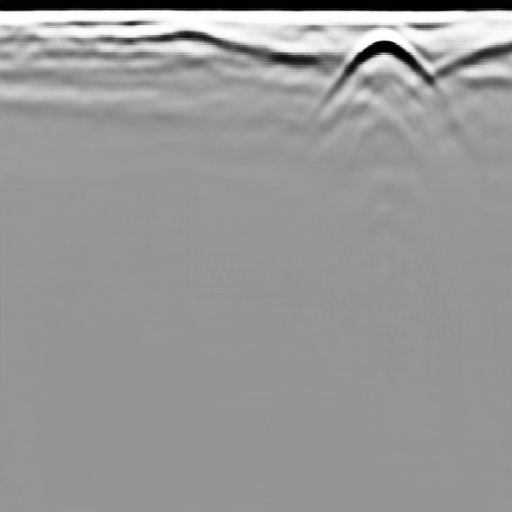
\includegraphics[width=\linewidth]{figures/high_res_gen.png}
    \caption{Generated A}
  \end{subfigure}
  \begin{subfigure}[b]{0.4\linewidth}
    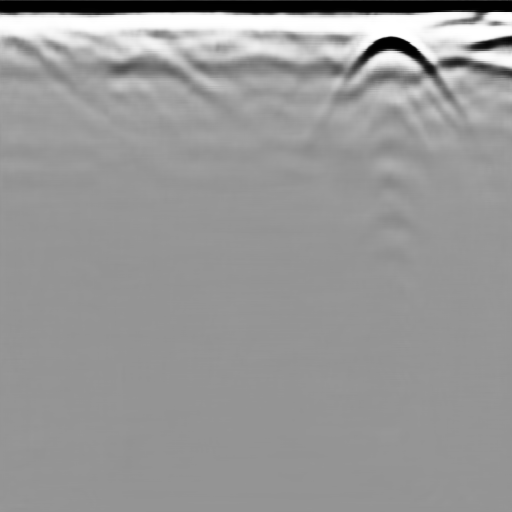
\includegraphics[width=\linewidth]{figures/high_res_gan_comparison.png}
    \caption{Generated B}
  \end{subfigure}
  \caption{Soil Variance Comparison in Similar B-scans}
  \label{fig:hi_res_compare}
\end{figure}

\subsection{Sample Diversity}\label{sample diversity}
An important discussion of generative results is the diversity of the samples. In Figure \ref{fig:real_diversity}, we can see that our generative model supplies a diverse set of samples. Note that the hyperbolas do not see much variation, this is the desired behavior. Moreover, one should pay special attention to how the noise changes between samples. Visually, not a single noise distribution is identical. In Section \ref{paradox}, we discussed a paradox when it comes to evaluating generative models. This paradox is especially important in sample diversity of unsupervised experiments which we do not have explicit class labels. The argument is that at what point are we simply memorizing the training distribution and how to define this point. Qualitatively, we see that our generative model does produce visually different images, but saying definitely that our model is not simply memorizing the training examples is a bit elusive. We do know that not a single identical image is produced, and that the images are visually realistic. However, exactly how close the images are to the training set is not quantitatively clear. The next section discusses the class conditioning results, which is a better approach to identify sample diversity. 

\begin{figure}[H]
    \centering
    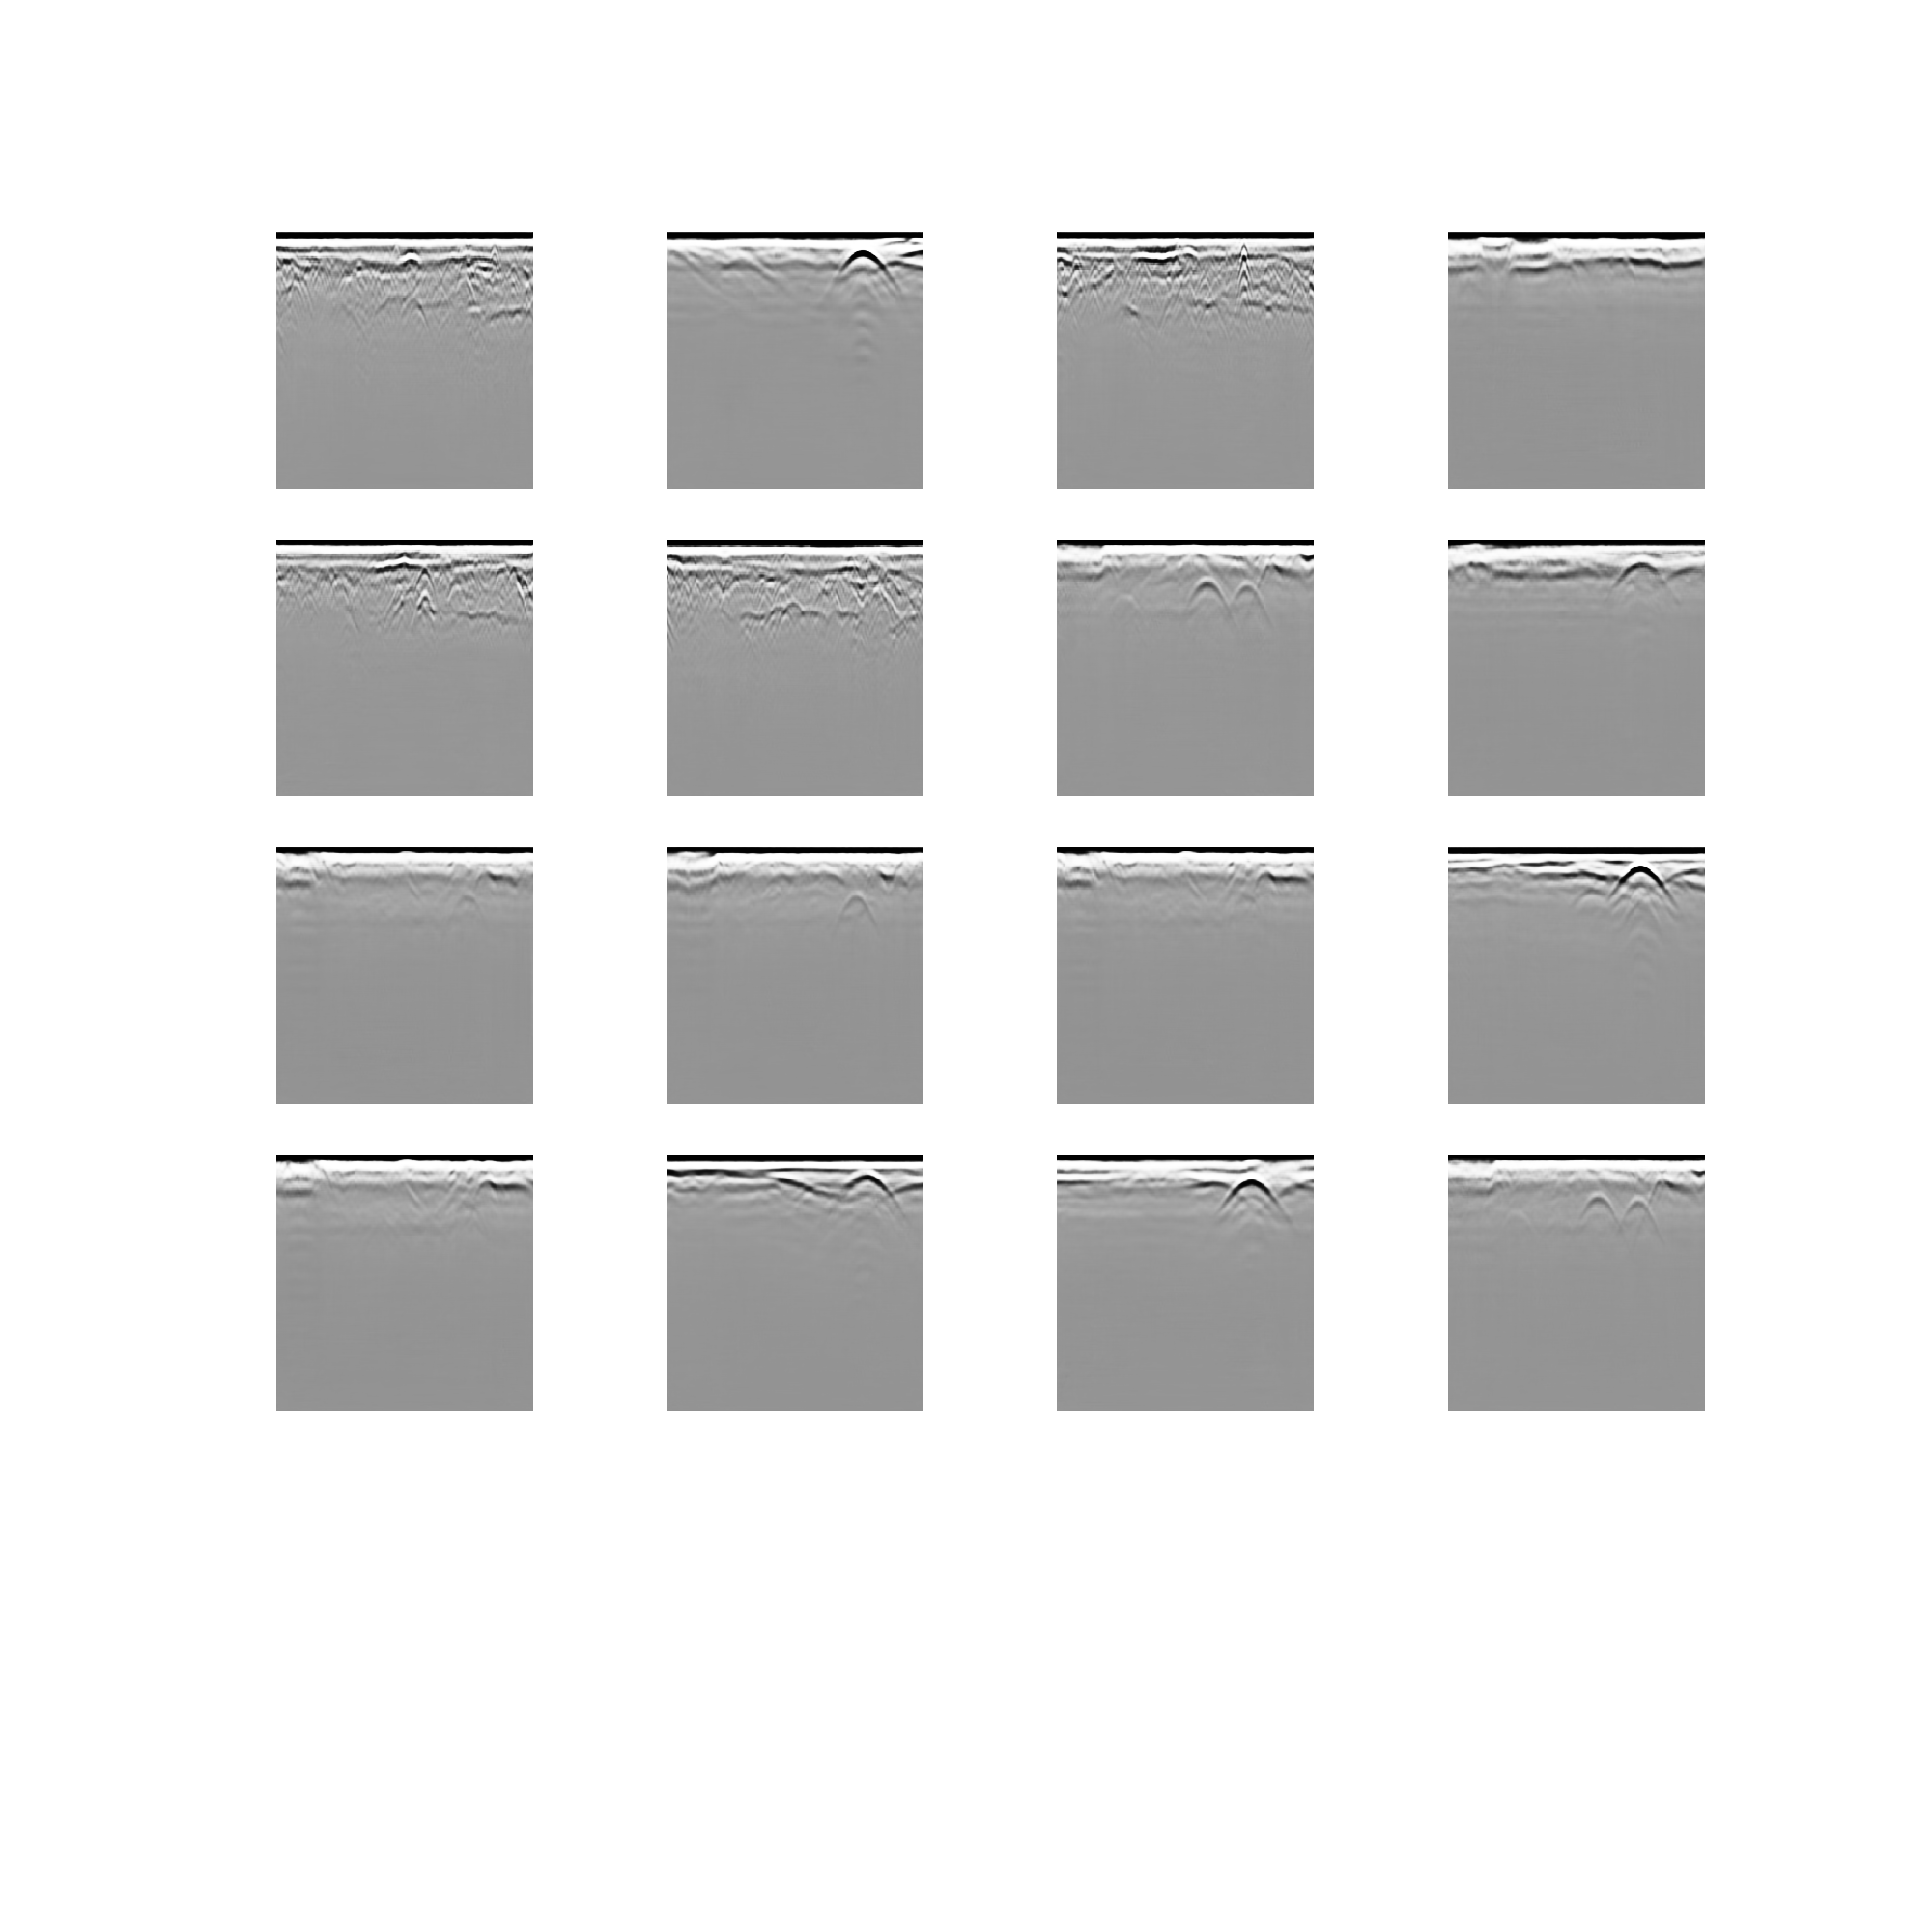
\includegraphics[width=\linewidth]{figures/diversity_512.png}
    \caption{Realistic Generated Images}
    \label{fig:real_diversity}
\end{figure}


\section{Supervised GAN Experiments}\label{Supervised}
In this section, we will look at the results of Supervised GAN Experiments. These are the set of experiments that contain class conditioning. This is only possible with the use of GprMax that allows us to simulate the material of the underground object and retain a definitive label. This is necessary in the classification task and also a major drawback of collected B-scans. In the field, B-scans that are collected do not have a ground truth class label due to the subjective nature of real B-scan evaluation. In this experiment, we can generate realistic type data that does have a definitive class label. Therefore, we are able to map a set of image features to the label. 

\subsection{Class Conditioning Examples}
Figure \ref{fig:image_compare} shows examples of the different classes that were the targets. The GAN model was able to learn distinct features of each class and then generate images of this type when given a label. An important note on continuation of this work is that ideally one would want to be able to combine the Unsupervised with the Supervised to generate a real B-scan with a known class. This is theoretically possible, however it is beyond the scope of this work. 

\begin{figure}[H]
  \centering
  \begin{subfigure}[b]{0.4\linewidth}
    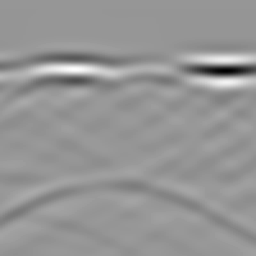
\includegraphics[width=\linewidth]{figures/sample_gprmax_bscan_concrete.png}
    \caption{Concrete}
  \end{subfigure}
  \begin{subfigure}[b]{0.4\linewidth}
    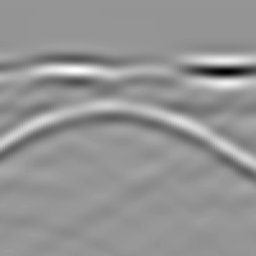
\includegraphics[width=\linewidth]{figures/metallic_bscan_gprmax.png}
    \caption{Metallic}
  \end{subfigure}
  \begin{subfigure}[b]{0.4\linewidth}
    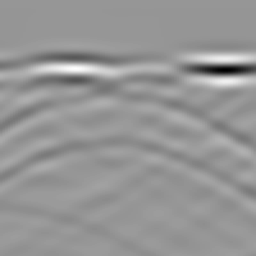
\includegraphics[width=\linewidth]{figures/sample_bscan_pvc.png}
    \caption{PVC}
  \end{subfigure}
  \caption{Generated B-scan of Each Class}
  \label{fig:image_compare}
\end{figure}

\subsection{Sample Diversity}
To demonstrate the diversity in samples, the reader is directed to Figure \ref{fig:grid}. As one can see the diversity compared to the unsupervised experiments, especially in the hyperbola, is greater. This is due to the ability of being able to control the exact location of the hyperbola. Therefore, in the simulation through GprMax we can make certain that there is maximum variability in the training data. Furthermore, we get interpolation between positions of the hyperbola. This effect is due to defining a range where the hyperbola can occur. Moreover, with multiple hyperbola positions the model can learn the probable location of where a hyperbolas can occur which is evident by the high variability of hyperbola location in the generated set. Another important aspect is that even though the hyperbola changes position, it does not change shape and retains the characteristics of the particular material class. This is of vital importance because any change in shape or visibility can be interpreted as a different object than the desired target one.

\begin{figure}[H]
    \centering
    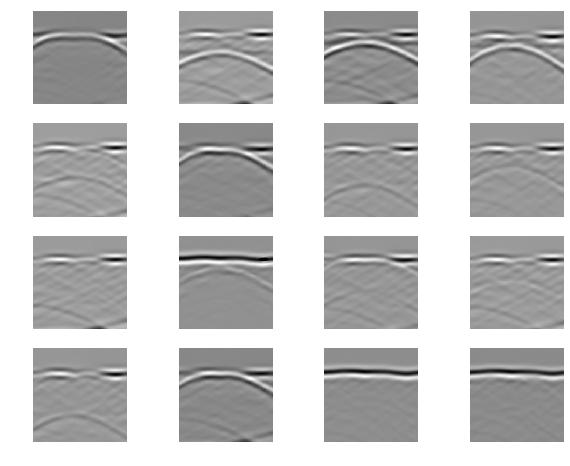
\includegraphics[width=\linewidth]{figures/generated_grid.png}
    \caption{Generated Time B-scans}
    \label{fig:grid}
\end{figure}

\subsection{Frequency Sample Diversity}
Figure \ref{fig:freq_grid} demonstrates the diversity in the generated Frequency B-scans. An important note is that these are not all of the possible variations, but a small subset for conciseness. In the frequency domain, we see that the model retains the ability to generate a wide array of features. Identical to the previous sections, we do not want to see variation in the hyperbola shape. Again, notice the noise variation, which ranges from very little noise in the background, to almost masking the hyperbola. This level of variation will be important in classifier evaluation.

\begin{figure}[H]
    \centering
    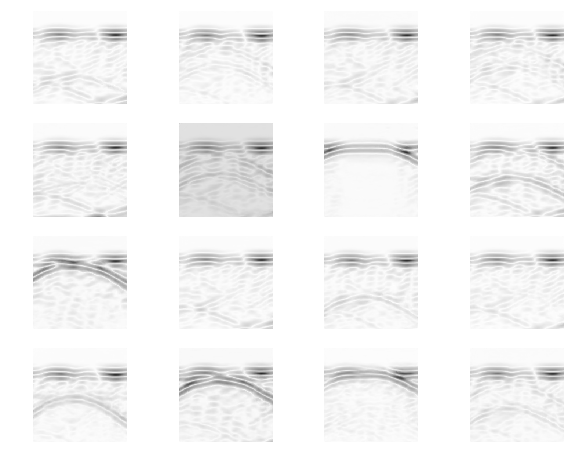
\includegraphics[width=\linewidth]{figures/freq_grid.png}
    \caption{Generated Frequency B-scans using Figure \ref{fig:tf-bscan}}
    \label{fig:freq_grid}
\end{figure}

\section{Object Identification Performance}
The following sections are the performance of the proposed classifier in each test scenario. The main objective is to demonstrate improvement in two places. We would like to see performance improvement with data augmentation via GAN generated images and further improvement when combining the time and frequency B-scans. 

\subsection{Time Domain}
For this set of experiments, we are only using time domain B-scans. These are the traditional B-scan representations that are present in the field collected examples presented in Section \ref{Unsupervised} and simulated in first part of Section \ref{Supervised}. Performance in this area is a key baseline to realized performance in the subsequent sections. 

\begin{table}[H]
\begin{center}
    Before Augmentation\\
    \begin{tabular}{ |c|c|c|c|c|c|c|}
        \hline
        Class & Accuracy & Precision & Recall & F1 & N \\
        \hline
        Concrete & 1.00 & 0.54 & 1.00 & 0.70 & 20\\ 
        Metallic & 0.81 & 1.00 & 0.82 & 0.90 & 11\\  
        PVC      & 0.50 & 0.67 & 0.57 & 0.62 & 14\\
        \hline
        All      & 0.77 & 0.74 & 0.80 & 0.75 & 45\\
        \hline
    \end{tabular} \\

    After Augmentation \\
    \begin{tabular}{ |c|c|c|c|c|c|}
        \hline
        Class & Accuracy & Precision & Recall & F1 & N \\
        \hline
        Concrete & 1.00 & 0.88 & 1.00 & 0.93 & 14\\ 
        Metallic & 0.91 & 1.00 & 0.91 & 0.95 & 11\\  
        PVC      & 0.90 & 0.95 & 0.90 & 0.92 & 20\\
        \hline
        All      & 0.94 & 0.94 & 0.94 & 0.93 & 45\\
        \hline
    \end{tabular}
\end{center}
\caption{Baseline Object Detection Performance}
\label{table:baseline}
\end{table}

From Table \ref{table:baseline}, we present the tabular results of the baseline performance. It is important to point out that these results are still in the upper half in regards to the performance metrics. However, as it will be demonstrated, there is still room for improvement. PVC is by far the worst performing material class. This is due to the lack of reflectivity in PVC cylinders. In Figure \ref{fig:image_compare}, it can be seen that PVC is visually, the least prominent hyperbola followed closely by concrete. From the results, this visibility difference translates to the classifier performance. Metallic, being the most visually prominent, is easily identified by the detection model. The lower portion of Table \ref{table:baseline} shows the performance achieved by training the classifier with augmented data. Overall, there is a performance increase when adding augmented training data. Most importantly, this is seen in the weak areas of the classifier. In the accuracy of PVC there is significant improvement that closes the gap between PVC and metallic cylinders. This means that when more samples are present in the training data that an overall increase in classifier performance will be realized.

\begin{figure}[H]
  \centering
  \begin{subfigure}[b]{0.4\linewidth}
    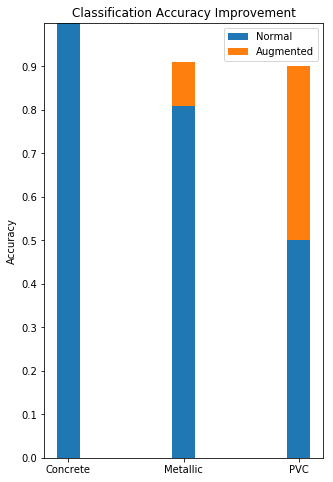
\includegraphics[width=\linewidth]{figures/Time-Accuracy.png}
    \caption{Accuracy}
  \end{subfigure}
  \begin{subfigure}[b]{0.4\linewidth}
    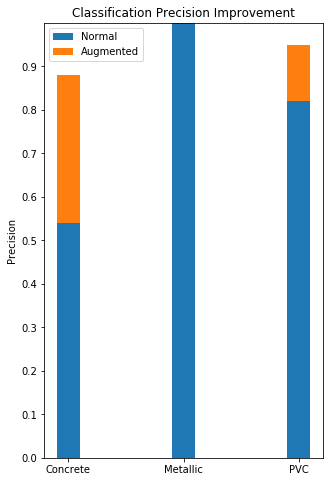
\includegraphics[width=\linewidth]{figures/Time-Precision.png}
    \caption{Precision}
  \end{subfigure}
  \begin{subfigure}[b]{0.4\linewidth}
    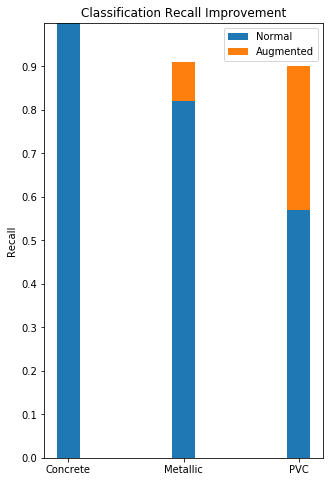
\includegraphics[width=\linewidth]{figures/Time-Recall.png}
    \caption{Recall}
  \end{subfigure}
  \begin{subfigure}[b]{0.4\linewidth}
    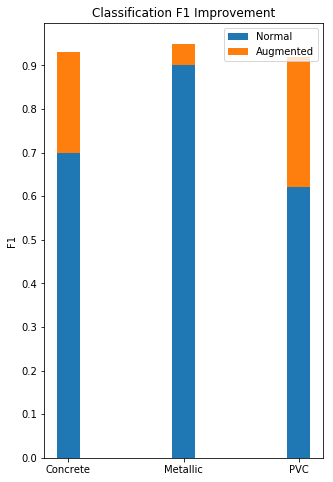
\includegraphics[width=\linewidth]{figures/Time-F1.png}
    \caption{F1}
  \end{subfigure}
  \caption{Time Results}
  \label{fig:time-results}
\end{figure}

Figure \ref{fig:time-results} is a visual representation of the performance improvement. The blue bar is the performance without augmentation and the orange is improvement factor with augmentation. The total bar height is the final result achieved in each performance metric. Note that for metallic cylinders performance does not have a large increase, but augmentation improved almost every metric for concrete and PVC cylinders. Next, we will see how the classifier performs in only the frequency domain.


\subsection{Frequency Domain}
The next section discusses a classifier only trained on frequency B-scans. This experiment was to determine if the frequency representation leads to better performance in a particular class.

\begin{table}[H]
\begin{center}
    Before Augmentation \\
    \begin{tabular}{ |c|c|c|c|c|c|}
        \hline
        Class & Accuracy & Precision & Recall & F1 & N \\
        \hline
        Concrete & 0.21 & 0.80 & 0.21 & 0.33 & 19\\ 
        Metallic & 0.18 & 1.00 & 0.62 & 0.77 & 16\\  
        PVC      & 0.20 & 0.75 & 0.90 & 0.51 & 10\\
        \hline
        All      & 0.20 & 0.86 & 0.58 & 0.54 & 45\\
        \hline
    \end{tabular}\\
    After Augmentation\\
    \begin{tabular}{ |c|c|c|c|c|c|}
        \hline
        Class & Accuracy & Precision & Recall & F1 & N \\
        \hline
        Concrete & 0.64 & 0.83 & 1.00 & 0.90 & 19\\ 
        Metallic & 0.36 & 1.00 & 0.88 & 0.93 & 16\\  
        PVC      & 0.60 & 1.00 & 0.60 & 0.67 & 10\\
        \hline
        All      & 0.53 & 0.94 & 0.83 & 0.83 & 45\\
        \hline
    \end{tabular}
\end{center}
\caption{Frequency Object Detection Performance}
\label{table:freq_table}
\end{table}

Table \ref{table:freq_table} contains the numerical performance results. The classification of PVC outperformed that of metallic in accuracy when using a frequency B-scan. The significance in this is that if frequency information is given to the classifier that the weakest class in the baseline is able to be detected at a better rate than the strongest performing baseline class. Notice that precision in the frequency domain is high in all of the classes. Recall is an additional area in which PVC performs well. Although, performance is not quite as good as the time domain classifier trained with augmented data. Next, let us look at how augmentation can improve performance in the frequency domain. The bottom half of \ref{table:freq_table} contains the metrics after augmentation. Overall, there is improvement in all metrics. 

\begin{figure}[H]
  \centering
  \begin{subfigure}[b]{0.4\linewidth}
    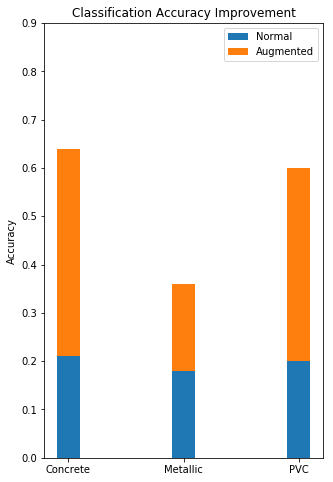
\includegraphics[width=\linewidth]{figures/Frequency-Accuracy.png}
    \caption{Accuracy}
  \end{subfigure}
  \begin{subfigure}[b]{0.4\linewidth}
    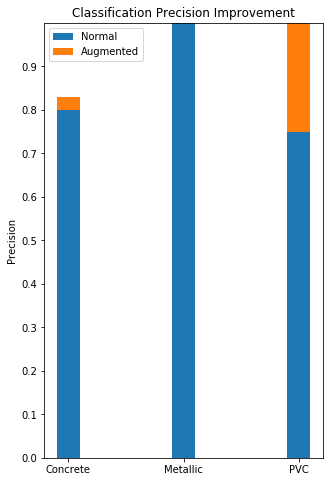
\includegraphics[width=\linewidth]{figures/Frequency-Precision.png}
    \caption{Precision}
  \end{subfigure}
  \begin{subfigure}[b]{0.4\linewidth}
    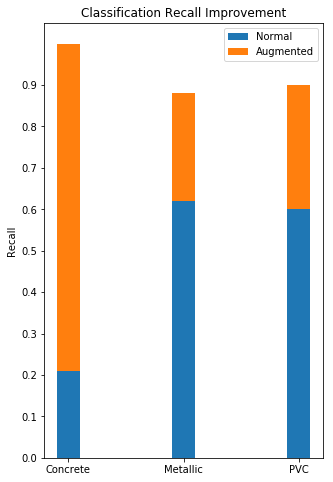
\includegraphics[width=\linewidth]{figures/Frequency-Recall.png}
    \caption{Recall}
  \end{subfigure}
  \begin{subfigure}[b]{0.4\linewidth}
    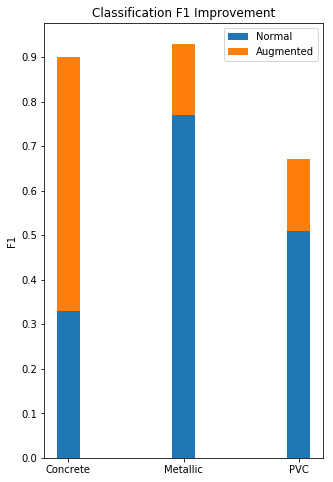
\includegraphics[width=\linewidth]{figures/Frequency-F1.png}
    \caption{F1}
  \end{subfigure}
  \caption{Frequency Results}
  \label{fig:freq-results}
\end{figure}

Figure \ref{fig:freq-results} is a visual demonstration of the improvement factor realized by using augmented data. An important area of improvement is in the Concrete class. Identification of Concrete was greatly improved by augmentation. Again, this is due to the improved detection ability that comes from using a frequency representation. This is evident when compared to the Metallic class. This class has the smallest improvement factor, because it was initially the best performing and also the most visible class. Finally, we will take a look at the performance when using a combined approach for material classification. 


\subsection{Combined Approach}
In the combined approach, we are using both time domain and frequency domain B-scans. This essentially is doubling the amount of features used for classification. As reviewed in previous sections, frequency representations allowed improvement for the weak areas of material classification. A combined approach will yield an improved classifier for all materials. 

\begin{table}[H]
\begin{center}
    Before Augmentation\\
    \begin{tabular}{ |c|c|c|c|c|c|}
        \hline
        Class & Accuracy & Precision & Recall & F1 & N \\
        \hline
        Concrete & 1.00 & 0.54 & 1.00 & 0.70 & 18\\ 
        Metallic & 0.91 & 1.00 & 0.93 & 0.96 & 14\\  
        PVC      & 0.55 & 1.00 & 0.69 & 0.62 & 13\\
        \hline
        All      & 0.82 & 0.85 & 0.87 & 0.76 & 45\\
        \hline
    \end{tabular}\\
    After Augmentation\\
    \begin{tabular}{ |c|c|c|c|c|c|}
        \hline
        Class & Accuracy & Precision & Recall & F1 & N \\
        \hline
        Concrete & 1.00 & 0.88 & 1.00 & 0.93 & 14\\ 
        Metallic & 1.00 & 1.00 & 1.00 & 1.00 & 11\\  
        PVC      & 0.95 & 1.00 & 0.90 & 0.95 & 20\\
        \hline
        All      & 0.98 & 0.96 & 0.97 & 0.96 & 45\\
        \hline
    \end{tabular}
\end{center}
\caption{Combined Object Detection Performance}
\label{table:combined_table}
\end{table}

Table \ref{table:combined_table}, depicts the classification scores achieved before the use of augmented data. Compared to the baseline, this approach realizes a significant increase in all evaluation metrics. Notice that PVC is still the worst performer in accuracy. However, it still sees an improvement from the baseline. This indicates that using a combined approach did improve the results of a weak class in accuracy. This is also true for the other metrics in relation to PVC. Concrete did not see an improvement from the baseline when adding features from the frequency domain. This is unusual due to the increased performance in all metrics from the frequency domain experiments. However, it is important to note that Concrete already achieved max values in accuracy and precision in the baseline test. Therefore, the improvement did not occur in precision only. The two other classes, Metallic and PVC, saw performance improvement in every metric with the combined approach. Thus meaning that a combined approach is superior to using only time domain or frequency domain features individually. Now, we will look at the effect augmentation had on the combined classifier performance.  

\begin{figure}[H]
  \centering
  \begin{subfigure}[b]{0.4\linewidth}
    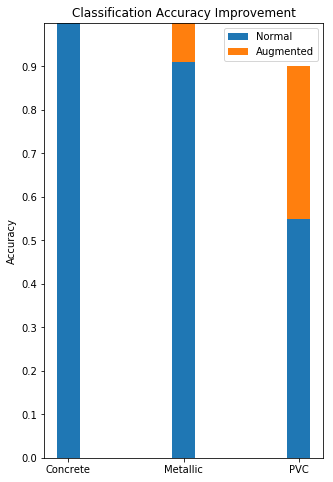
\includegraphics[width=\linewidth]{figures/Combined-Accuracy.png}
    \caption{Accuracy}
  \end{subfigure}
  \begin{subfigure}[b]{0.4\linewidth}
    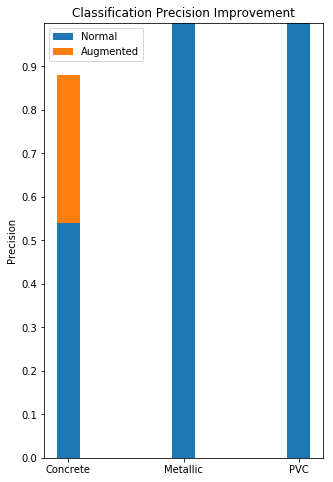
\includegraphics[width=\linewidth]{figures/Combined-Precision.png}
    \caption{Precision}
  \end{subfigure}
  \begin{subfigure}[b]{0.4\linewidth}
    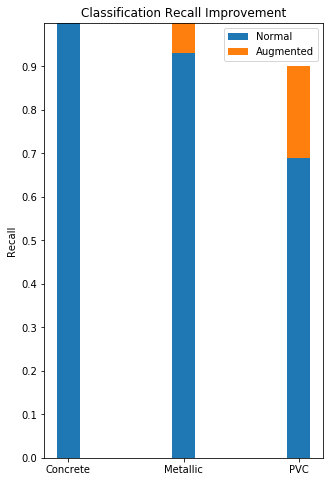
\includegraphics[width=\linewidth]{figures/Combined-Recall.png}
    \caption{Recall}
  \end{subfigure}
  \begin{subfigure}[b]{0.4\linewidth}
    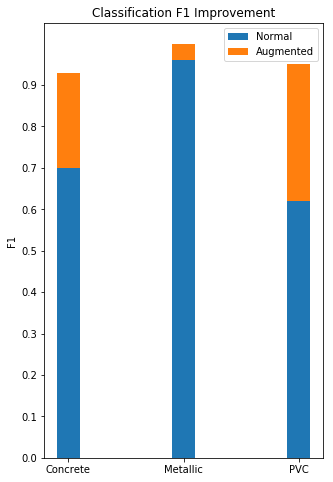
\includegraphics[width=\linewidth]{figures/Combined-F1.png}
    \caption{F1}
  \end{subfigure}
  \caption{Combined Results}
  \label{fig:combined-results}
\end{figure}

Figure \ref{fig:combined-results}, shows the improvement factor of adding augmented data. The improvement factor is smallest among all of the experiments. This is due to the already significant performance increase from incorporating frequency domain features. Continuing the previous trends, PVC is the weakest and also enjoys the most performance improvement from augmented data. 

\section{Summary}
In conclusion, it was demonstrated that \acrshort{gan} could be successfully applied to \acrshort{gpr} data. This is shown in both real and simulated B-scans. In addition, we looked at how the class conditioning could be applied to \acrshort{gan} to generate labeled training data for a classifier. With this training data, it was shown that \acrshort{gan} augmentation can improve a classifier. Furthermore, frequency domain features can be applied in a combined classifier, which enabled an additional boost in the scoring metrics for the classifier.